\documentclass{standalone}
\usepackage{tikz}
\usetikzlibrary{patterns, positioning}


\begin{document}
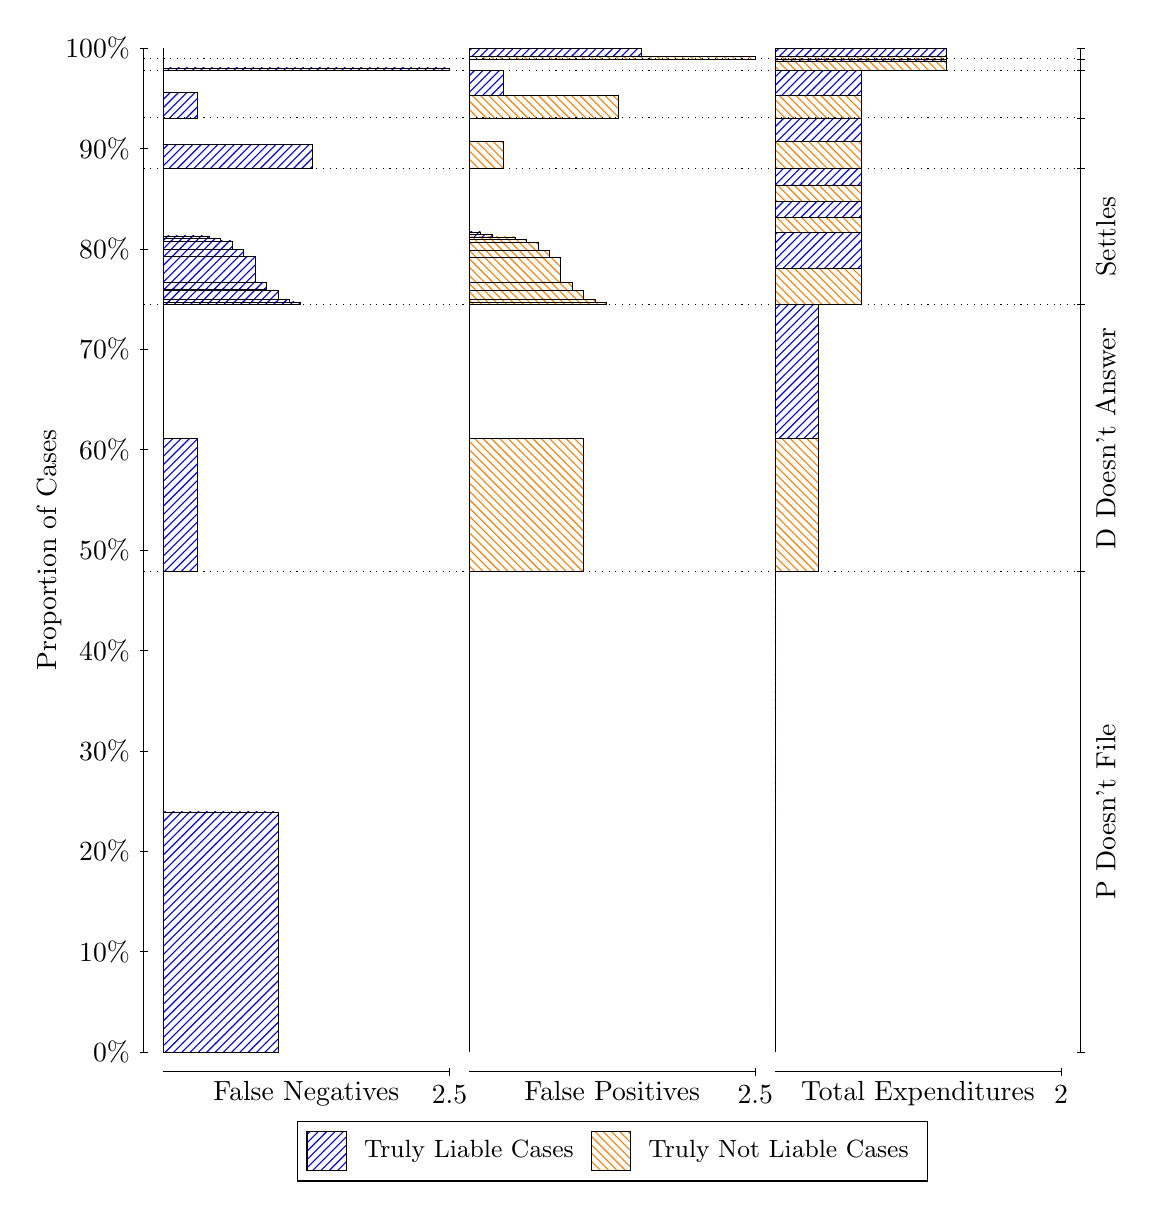
\begin{tikzpicture}
\draw[black, very thin] (1.5,1.75) -- (1.5,14.5);
\node[rotate=90, text=black, anchor=center] at (0.3, 8.125) {Proportion of Cases};
\draw[black, very thin] (1.45,1.75) -- (1.55,1.75);
\node[text=black, anchor=east] at (1.45, 1.75) {0\%};
\draw[black, very thin] (1.45,3.025) -- (1.55,3.025);
\node[text=black, anchor=east] at (1.45, 3.025) {10\%};
\draw[black, very thin] (1.45,4.3) -- (1.55,4.3);
\node[text=black, anchor=east] at (1.45, 4.3) {20\%};
\draw[black, very thin] (1.45,5.575) -- (1.55,5.575);
\node[text=black, anchor=east] at (1.45, 5.575) {30\%};
\draw[black, very thin] (1.45,6.85) -- (1.55,6.85);
\node[text=black, anchor=east] at (1.45, 6.85) {40\%};
\draw[black, very thin] (1.45,8.125) -- (1.55,8.125);
\node[text=black, anchor=east] at (1.45, 8.125) {50\%};
\draw[black, very thin] (1.45,9.4) -- (1.55,9.4);
\node[text=black, anchor=east] at (1.45, 9.4) {60\%};
\draw[black, very thin] (1.45,10.675) -- (1.55,10.675);
\node[text=black, anchor=east] at (1.45, 10.675) {70\%};
\draw[black, very thin] (1.45,11.95) -- (1.55,11.95);
\node[text=black, anchor=east] at (1.45, 11.95) {80\%};
\draw[black, very thin] (1.45,13.225) -- (1.55,13.225);
\node[text=black, anchor=east] at (1.45, 13.225) {90\%};
\draw[black, very thin] (1.45,14.5) -- (1.55,14.5);
\node[text=black, anchor=east] at (1.45, 14.5) {100\%};

\draw[black, very thin] (13.4,1.75) -- (13.4,14.5);
\draw[black, very thin] (13.35,1.75) -- (13.45,1.75);
\node[anchor=west] at (13.35, 1.75) {};
\draw[black, very thin] (13.35,7.8487) -- (13.45,7.8487);
\node[anchor=west] at (13.35, 7.8487) {};
\draw[black, very thin] (13.35,11.24) -- (13.45,11.24);
\node[anchor=west] at (13.35, 11.24) {};
\draw[black, very thin] (13.35,12.974) -- (13.45,12.974);
\node[anchor=west] at (13.35, 12.974) {};
\draw[black, very thin] (13.35,13.613) -- (13.45,13.613);
\node[anchor=west] at (13.35, 13.613) {};
\draw[black, very thin] (13.35,14.22) -- (13.45,14.22);
\node[anchor=west] at (13.35, 14.22) {};
\draw[black, very thin] (13.35,14.363) -- (13.45,14.363);
\node[anchor=west] at (13.35, 14.363) {};
\draw[black, very thin] (13.35,14.5) -- (13.45,14.5);
\node[anchor=west] at (13.35, 14.5) {};

\draw[black, very thin, pattern color=blue, pattern=north east lines] (1.75,1.75) rectangle (3.2033,4.7993);
\draw[black, very thin, pattern color=orange, pattern=north west lines] (1.75,4.7993) rectangle (1.75,7.8487);
\draw[black, very thin, pattern color=blue, pattern=north east lines] (1.75,7.8487) rectangle (2.186,9.5443);
\draw[black, very thin, pattern color=orange, pattern=north west lines] (1.75,9.5443) rectangle (1.75,11.24);
\draw[black, very thin, pattern color=blue, pattern=north east lines] (1.75,11.24) rectangle (3.494,11.275);
\draw[black, very thin, pattern color=blue, pattern=north east lines] (1.75,11.275) rectangle (3.3487,11.307);
\draw[black, very thin, pattern color=blue, pattern=north east lines] (1.75,11.307) rectangle (3.2033,11.421);
\draw[black, very thin, pattern color=blue, pattern=north east lines] (1.75,11.421) rectangle (3.058,11.442);
\draw[black, very thin, pattern color=blue, pattern=north east lines] (1.75,11.442) rectangle (3.058,11.526);
\draw[black, very thin, pattern color=blue, pattern=north east lines] (1.75,11.526) rectangle (2.9127,11.852);
\draw[black, very thin, pattern color=blue, pattern=north east lines] (1.75,11.852) rectangle (2.7673,11.947);
\draw[black, very thin, pattern color=blue, pattern=north east lines] (1.75,11.947) rectangle (2.622,12.05);
\draw[black, very thin, pattern color=blue, pattern=north east lines] (1.75,12.05) rectangle (2.4767,12.079);
\draw[black, very thin, pattern color=blue, pattern=north east lines] (1.75,12.079) rectangle (2.3313,12.113);
\draw[black, very thin, pattern color=orange, pattern=north west lines] (1.75,12.113) rectangle (1.75,12.974);
\draw[black, very thin, pattern color=blue, pattern=north east lines] (1.75,12.974) rectangle (3.6393,13.272);
\draw[black, very thin, pattern color=orange, pattern=north west lines] (1.75,13.272) rectangle (1.75,13.613);
\draw[black, very thin, pattern color=blue, pattern=north east lines] (1.75,13.613) rectangle (2.186,13.935);
\draw[black, very thin, pattern color=orange, pattern=north west lines] (1.75,13.935) rectangle (1.75,14.22);
\draw[black, very thin, pattern color=blue, pattern=north east lines] (1.75,14.22) rectangle (5.3833,14.247);
\draw[black, very thin, pattern color=orange, pattern=north west lines] (1.75,14.247) rectangle (1.75,14.363);
\draw[black, very thin, pattern color=orange, pattern=north west lines] (1.75,14.363) rectangle (1.75,14.391);
\draw[black, very thin, pattern color=blue, pattern=north east lines] (1.75,14.391) rectangle (1.75,14.5);
\draw[black, very thin, pattern color=orange, pattern=north west lines] (5.6333,1.75) rectangle (5.6333,4.7994);
\draw[black, very thin, pattern color=blue, pattern=north east lines] (5.6333,4.7994) rectangle (5.6333,7.8487);
\draw[black, very thin, pattern color=orange, pattern=north west lines] (5.6333,7.8487) rectangle (7.0867,9.5443);
\draw[black, very thin, pattern color=blue, pattern=north east lines] (5.6333,9.5443) rectangle (5.6333,11.24);
\draw[black, very thin, pattern color=orange, pattern=north west lines] (5.6333,11.24) rectangle (7.3773,11.274);
\draw[black, very thin, pattern color=orange, pattern=north west lines] (5.6333,11.274) rectangle (7.232,11.305);
\draw[black, very thin, pattern color=orange, pattern=north west lines] (5.6333,11.305) rectangle (7.0867,11.42);
\draw[black, very thin, pattern color=orange, pattern=north west lines] (5.6333,11.42) rectangle (6.9413,11.525);
\draw[black, very thin, pattern color=orange, pattern=north west lines] (5.6333,11.525) rectangle (6.796,11.842);
\draw[black, very thin, pattern color=orange, pattern=north west lines] (5.6333,11.842) rectangle (6.6507,11.933);
\draw[black, very thin, pattern color=orange, pattern=north west lines] (5.6333,11.933) rectangle (6.5053,12.034);
\draw[black, very thin, pattern color=orange, pattern=north west lines] (5.6333,12.034) rectangle (6.36,12.066);
\draw[black, very thin, pattern color=orange, pattern=north west lines] (5.6333,12.066) rectangle (6.2147,12.101);
\draw[black, very thin, pattern color=blue, pattern=north east lines] (5.6333,12.101) rectangle (5.924,12.135);
\draw[black, very thin, pattern color=blue, pattern=north east lines] (5.6333,12.135) rectangle (5.7787,12.165);
\draw[black, very thin, pattern color=blue, pattern=north east lines] (5.6333,12.165) rectangle (5.6333,12.974);
\draw[black, very thin, pattern color=orange, pattern=north west lines] (5.6333,12.974) rectangle (6.0693,13.316);
\draw[black, very thin, pattern color=blue, pattern=north east lines] (5.6333,13.316) rectangle (5.6333,13.613);
\draw[black, very thin, pattern color=orange, pattern=north west lines] (5.6333,13.613) rectangle (7.5227,13.897);
\draw[black, very thin, pattern color=blue, pattern=north east lines] (5.6333,13.897) rectangle (6.0693,14.22);
\draw[black, very thin, pattern color=orange, pattern=north west lines] (5.6333,14.22) rectangle (5.6333,14.336);
\draw[black, very thin, pattern color=blue, pattern=north east lines] (5.6333,14.336) rectangle (5.6333,14.363);
\draw[black, very thin, pattern color=orange, pattern=north west lines] (5.6333,14.363) rectangle (9.2667,14.391);
\draw[black, very thin, pattern color=blue, pattern=north east lines] (5.6333,14.391) rectangle (7.8133,14.5);
\draw[black, very thin, pattern color=orange, pattern=north west lines] (9.5167,1.75) rectangle (9.5167,4.7994);
\draw[black, very thin, pattern color=blue, pattern=north east lines] (9.5167,4.7994) rectangle (9.5167,7.8487);
\draw[black, very thin, pattern color=orange, pattern=north west lines] (9.5167,7.8487) rectangle (10.062,9.5443);
\draw[black, very thin, pattern color=blue, pattern=north east lines] (9.5167,9.5443) rectangle (10.062,11.24);
\draw[black, very thin, pattern color=orange, pattern=north west lines] (9.5167,11.24) rectangle (10.607,11.703);
\draw[black, very thin, pattern color=blue, pattern=north east lines] (9.5167,11.703) rectangle (10.607,12.161);
\draw[black, very thin, pattern color=orange, pattern=north west lines] (9.5167,12.161) rectangle (10.607,12.35);
\draw[black, very thin, pattern color=blue, pattern=north east lines] (9.5167,12.35) rectangle (10.607,12.553);
\draw[black, very thin, pattern color=orange, pattern=north west lines] (9.5167,12.553) rectangle (10.607,12.762);
\draw[black, very thin, pattern color=blue, pattern=north east lines] (9.5167,12.762) rectangle (10.607,12.974);
\draw[black, very thin, pattern color=orange, pattern=north west lines] (9.5167,12.974) rectangle (10.607,13.316);
\draw[black, very thin, pattern color=blue, pattern=north east lines] (9.5167,13.316) rectangle (10.607,13.613);
\draw[black, very thin, pattern color=orange, pattern=north west lines] (9.5167,13.613) rectangle (10.607,13.897);
\draw[black, very thin, pattern color=blue, pattern=north east lines] (9.5167,13.897) rectangle (10.607,14.22);
\draw[black, very thin, pattern color=orange, pattern=north west lines] (9.5167,14.22) rectangle (11.697,14.336);
\draw[black, very thin, pattern color=blue, pattern=north east lines] (9.5167,14.336) rectangle (11.697,14.363);
\draw[black, very thin, pattern color=orange, pattern=north west lines] (9.5167,14.363) rectangle (11.697,14.391);
\draw[black, very thin, pattern color=blue, pattern=north east lines] (9.5167,14.391) rectangle (11.697,14.5);
\draw[black, dotted] (1.5,7.8487) -- (13.4,7.8487);
\draw[black, dotted] (1.5,11.24) -- (13.4,11.24);
\draw[black, dotted] (1.5,12.974) -- (13.4,12.974);
\draw[black, dotted] (1.5,13.613) -- (13.4,13.613);
\draw[black, dotted] (1.5,14.22) -- (13.4,14.22);
\draw[black, dotted] (1.5,14.363) -- (13.4,14.363);
\draw[black, very thin] (1.75,1.5) -- (5.3833,1.5);
\node[text=black, anchor=north] at (3.5667, 1.5) {False Negatives};
\draw[black, very thin] (5.3833,1.45) -- (5.3833,1.55);
\node[text=black, anchor=north] at (5.3833, 1.45) {2.5};

\draw[black, very thin] (5.6333,1.5) -- (9.2667,1.5);
\node[text=black, anchor=north] at (7.45, 1.5) {False Positives};
\draw[black, very thin] (9.2667,1.45) -- (9.2667,1.55);
\node[text=black, anchor=north] at (9.2667, 1.45) {2.5};

\draw[black, very thin] (9.5167,1.5) -- (13.15,1.5);
\node[text=black, anchor=north] at (11.333, 1.5) {Total Expenditures};
\draw[black, very thin] (13.15,1.45) -- (13.15,1.55);
\node[text=black, anchor=north] at (13.15, 1.45) {2};

\node[text=black, centered, rotate=90] at (13.72, 4.7994) {P Doesn't File};
\node[text=black, centered, rotate=90] at (13.72, 9.5443) {D Doesn't Answer};
\node[text=black, centered, rotate=90] at (13.72, 12.107) {Settles};





\draw (7.449999999999999,1.5) node[draw=none] (baseCoordinate) {};
\begin{scope}[align=center]
        \matrix[scale=0.5, draw=black, below=0.5cm of baseCoordinate, nodes={draw}, column sep=0.1cm]{
            \node[rectangle, draw, minimum width=0.5cm, minimum height=0.5cm, pattern color=blue, pattern=north east lines] {}; &
            \node[draw=none, font=\small, text=black] (B) {Truly Liable Cases}; &
            \node[rectangle, draw, minimum width=0.5cm, minimum height=0.5cm, pattern color=orange, pattern=north west lines] {}; &
            \node[draw=none, font=\small, text=black] (B) {Truly Not Liable Cases}; \\
            };
\end{scope}

\end{tikzpicture}
\end{document}